\documentclass[12pt,fleqn]{article}

\usepackage[cp1251, utf8x]{inputenc}
\usepackage[T2A]{fontenc}
\usepackage{amssymb, amsmath, mathrsfs, amsthm}
\usepackage[russian]{babel}
\usepackage[footnotesize]{caption2}
\usepackage{indentfirst}
\usepackage{graphicx}
\usepackage[noend]{algorithmic}
\usepackage{algorithm}
\usepackage{color}
\usepackage{hyperref}
\usepackage{array}
    
\hypersetup{
	colorlinks = true,
	urlcolor = blue
}

\newcolumntype{L}[1]{>{\raggedright\let\newline\\\arraybackslash\hspace{0pt}}m{#1}}
\newcolumntype{C}[1]{>{\centering\let\newline\\\arraybackslash\hspace{0pt}}m{#1}}
\newcolumntype{R}[1]{>{\raggedleft\let\newline\\\arraybackslash\hspace{0pt}}m{#1}}

\begin{document}
\begin{titlepage}
\begin{center}
    Московский государственный университет имени М. В. Ломоносова

    \bigskip
    \includegraphics[width=50mm]{msu.eps}

    \bigskip
    Факультет Вычислительной математики и Кибернетики\\
  	Кафедра Математических Методов Прогнозирования\\[10mm]

	\textsf{\large\bfseries
        Обработка и методы распознавания изображений
    }\\[10mm]
    \textsf{\large\bfseries
        Отчет по лабораторной работе №2
    }\\[10mm]
	
	\bigskip
	\bigskip
	\bigskip
	\bigskip
	\bigskip
	\bigskip
	\bigskip
	\bigskip
	\bigskip
	
    \begin{flushright}
        \parbox{0.5\textwidth}{
            Выполнил:\\
            студент 3 курса 317 группы\\
            \emph{Таскынов Ануар}\\[5mm]
        }
    \end{flushright}

    \vspace{\fill}
    Москва, 2016
\end{center}
\end{titlepage}

\newpage
\renewcommand{\contentsname}{Содержание.}
\tableofcontents
\newpage
\section{Постановка задания.}

В данном задании необходимо было разработать программу для классификации изображений ладоней, по сгенерированным признакам. В качестве признакового описания строилась <<линия пальцев>>, соединяющая основания пальцев с их кончиками. 

Язык программирования Python 2. В качестве сторонней библиотеки использовалась библиотека компьютерного зрения OpenCV.  Эксперименты приведены в Ipython Notebook'е, функции описаны в отдельном python-модуле. Выполнен уровень Expert.

В уровне Expert помимо генерации признаков, необходимо было провести кластеризацию изображений.

\newpage
\section{Описание решения.}
\subsection{Бинаризация.}
Первым делом необходимо бинаризовать изображение. Это делалось следующим образом:
\begin{itemize}
\item Проводилась бинаризация по методу Оцу.
\item Найденный порог $t$ умножался на $1.6$. Это было сделано для того, чтобы полностью отделить руку от фона, так как некоторые изображения при пороге $t$ отделялись не полностью. Примеры показаны на рис. \hyperref[Image1]{1}
\item Дальше удаляются мелкие объекты.
\end{itemize}

\begin{figure}[h]
\begin{minipage}[h]{0.49\linewidth}
\center{
\includegraphics[width=0.95\linewidth]{bad_binary12} \\ Изображение 012} 
\end{minipage}
\hfill
\begin{minipage}[h]{0.49\linewidth}
\center{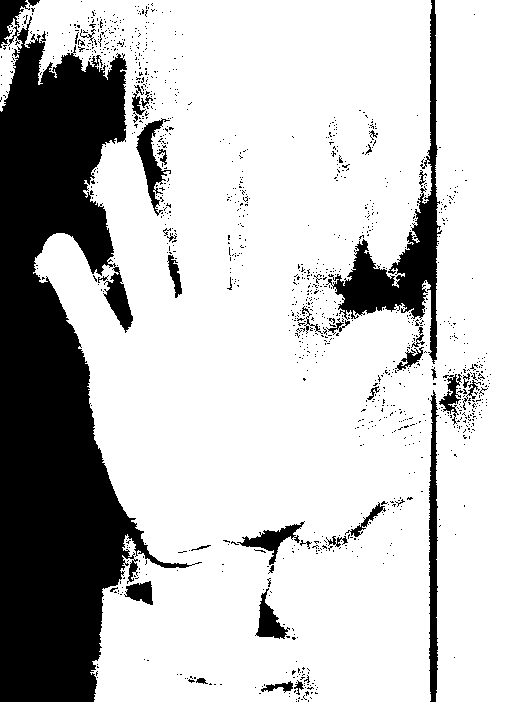
\includegraphics[width=0.95\linewidth]{bad_binary13} \\ Изображение 013} 
\end{minipage}
\caption{Изображения, на которых плохо отработал порог $t$.}
\label{Image1}
\end{figure}

При умножении порога на $1.6$ бинаризация значительно улучшается. Пример отработанной бинаризации на тех же изображениях показан на рис. \hyperref[Image2]{2}

\begin{figure}[h]
\begin{minipage}[h]{0.49\linewidth}
\center{
\includegraphics[width=0.95\linewidth]{binary12} \\ Изображение 012} 
\end{minipage}
\hfill
\begin{minipage}[h]{0.49\linewidth}
\center{
\includegraphics[width=0.95\linewidth]{binary13} \\ Изображение 013} 
\end{minipage}
\caption{Изображения, на которых плохо отработал порог $1.6t$.}
\label{Image2}
\end{figure}

\subsection{Выделение и фильтрация дефектов выпуклой оболочки.}

Дальше пойдет этап выделения дефектов выпуклой оболочки. Дефекты будут показывать на точки, куда было добавлено точек для создания выпуклой оболочки. Далее за start, far, end будут обозначаться начало дефекта, сам дефект, конец дефекта.

\begin{itemize}
\item Ищутся дефекты выпуклой оболочки.
\item Ищется угол между точками start, far и end. Так как угол между пальцами в основном острый, брался угол равный 95 для отсечения ненужных дефектов.
\item Также были замечены мелкие дефекты, которые также имеют острый угол. Для их отсечения считалась площадь треугольника на этих трех точках.
\end{itemize} 

\begin{figure}[h]
\center{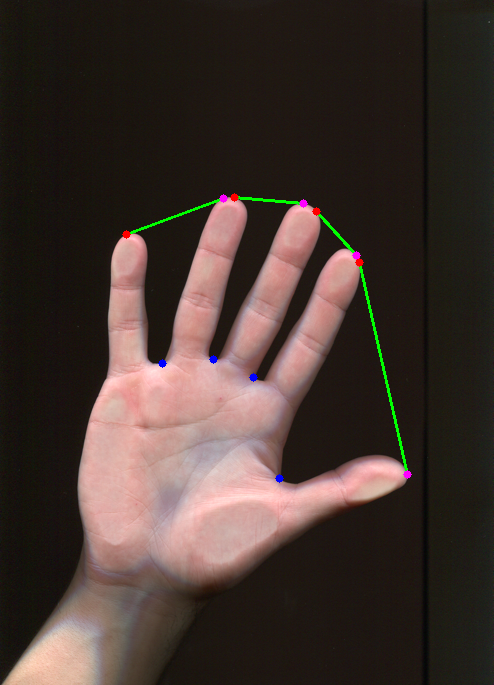
\includegraphics[width=0.4\linewidth]{defects_1}}
\caption{Начало дефекта указано красным цветом, сам дефект синим, конец дефекта розовым.}
\label{Image3}
\end{figure}

В результате проделанных манипуляций оставалось крайне мало дефектов не похожих на кончики пальцев и их основания. Но этого было не достаточно для полного отсечения ненужных дефектов (рис. \hyperref[Image4]{4}). Для их фильтрации использовалось следующее:

\begin{itemize}
\item С помощью метода distans transform ищется центр ладони.
\item Считаются все векторы, идущие с центра ладони и до дефекта. Дальше они ортонормируются.
\item Среди посчитанных векторов ищется средний.
\item Те вектора, образующие тупой угол со средним отсекаются.
\end{itemize}

Результат на рис. \hyperref[Image4]{4}.

\begin{figure}[h]
\begin{minipage}[h]{0.49\linewidth}
\center{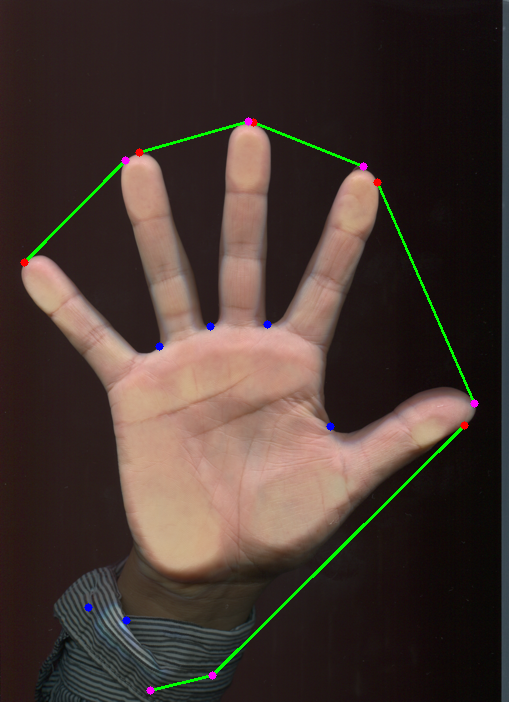
\includegraphics[width=0.7\linewidth]{bad_defects} \\ До фильтрации дефектов} 
\end{minipage}
\hfill
\begin{minipage}[h]{0.49\linewidth}
\center{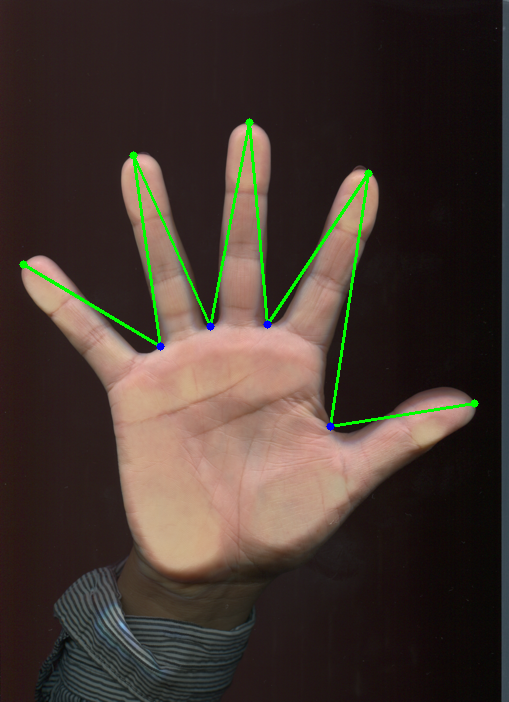
\includegraphics[width=0.7\linewidth]{defects_2} \\ После фильтрации дефектов.} 
\end{minipage}
\caption{Дефекты до и после фильтрации.}
\label{Image4}
\end{figure}

\subsection{Поиск большого пальца.}
Были сохранены начало и конец дефекта. Конец одного дефекта - это начало другого. Усредняя их мы получаем точку на кончике пальца. Далее, для того, чтобы определить большой палец выполнялось следующее:
\begin{itemize}
\item Проверялось условие того, что конец одного дефекта - это начало другого. Если нарушено это условие, то мы на границе (либо мизинец, либо большой палец). Таким образом можно отсортировать дефекты так, чтобы первым был дефект, отвечающий либо за мизинец, либо за большой палец.
\item Длина между основанием мизинца кончиком безымянного пальца меньше, чем расстояние между основанием большого пальца и указательного. Эта информация использовалась для того, чтобы найти большой палец.
\end{itemize}

Результат работы на рис. \hyperref[Image4]{4}. Таким образом сформировался вектор признаков для ладоней. Дальше идет кластеризация.
 
\newpage
\section{Кластеризация и результаты.}

Кластеризация проводилась методом K-средних. Для разного числа кластеров был нарисован график зависимости между числом кластеров и функционалом качества. Подробнее на рис. \hyperref[Image5]{5}.

\begin{figure}[h]
\center{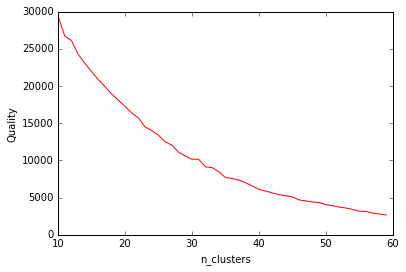
\includegraphics[width=1.0\linewidth]{clustering}}
\caption{График зависимости.}
\label{Image5}
\end{figure}

Как видно из графика, что чем больше количество кластеров, тем лучше качество, однако это сводится к переобучению. Поэтому было выбрано число кластеров равное $33$. Результаты на Табл. \hyperref[tabular2]{2}. Результаты поиска близких ладоней на Табл. \hyperref[tabular1]{1}

\newpage
\begin{table}[h]
\begin{center}
\begin{tabular}{|c|c|c|c|c|c|}
\hline
Имя образца & Соседи & Имя образца & Соседи & Имя образца & Соседи \\ \hline
         001 &            002 037 090  &         039 &            037 002 001  &         095 &            109 008 067  \\ 
         002 &            001 037 145  &         041 &            060 105 049  &         096 &            063 093 031  \\
        003 &            006 007 005  &         046 &            020 018 016  &         097 &            007 003 014  \\
        004 &            006 003 007  &         047 &            050 060 146  &         099 &            012 014 003  \\
         005 &            007 003 006  &         049 &            047 060 041  &         105 &            142 107 106  \\
        006 &            003 004 007  &         050 &            047 060 146  &         106 &            142 105 107  \\
         007 &            005 003 155  &         051 &            052 054 053  &         107 &            105 088 091  \\
        008 &            067 066 057  &         052 &            051 054 053  &         109 &            092 067 113  \\
         009 &            011 010 065  &         053 &            054 052 051  &         111 &            096 031 063  \\
        010 &            009 011 065  &         054 &            051 052 078  &         112 &            114 113 092  \\
         011 &            079 009 081  &         055 &            053 052 106  &         113 &            114 112 092  \\
         012 &            014 013 006  &         056 &            086 076 057  &         114 &            112 113 092  \\
         013 &            012 014 015  &         057 &            076 056 081  &         118 &            123 122 113  \\
         014 &            012 013 006  &         060 &            047 145 050  &         120 &            124 034 028  \\
        015 &            013 005 014  &         063 &            096 034 066  &         122 &            123 092 026  \\
         016 &            017 020 046  &         064 &            141 066 009  &         123 &            122 118 092  \\
        017 &            016 020 046  &         065 &            009 010 155  &         124 &            034 120 028  \\
         018 &            021 019 020  &         066 &            128 129 011  &         126 &            127 124 120  \\
         019 &            021 018 078  &         067 &            008 109 129  &         127 &            126 122 123  \\
        020 &            046 018 016  &         068 &            020 011 079  &         128 &            129 066 079  \\
        021 &            019 018 020  &         071 &            150 151 050  &         129 &            128 066 008  \\
        022 &            023 035 026  &         076 &            077 079 086  &         135 &            003 157 107  \\
         023 &            022 035 124  &         077 &            076 079 086  &         138 &            141 065 064  \\
         024 &            086 021 079  &         078 &            077 076 079  &         141 &            009 064 065  \\
        026 &            028 029 022  &         079 &            076 077 011  &         142 &            105 106 107  \\
         027 &            029 028 036  &         081 &            079 086 082  &         144 &            004 145 146  \\
         028 &            026 124 029  &         082 &            090 081 007  &         145 &            144 146 002  \\
         029 &            027 028 026  &         086 &            077 079 076  &         146 &            004 144 006  \\
         031 &            063 096 009  &         088 &            091 107 157  &         150 &            151 152 071  \\
         034 &            124 120 028  &         090 &            082 005 007  &         151 &            150 152 071  \\
         035 &            022 023 026  &         091 &            088 107 105  &         152 &            150 151 071  \\
         036 &            035 120 028  &         092 &            112 114 113  &         155 &            007 006 005  \\
         037 &            002 001 039  &         093 &            096 063 092  &         157 &            107 086 155  \\ \hline
\end{tabular}
\caption{Таблица ближайших соседей.}
\label{tabular1}
\end{center}
\end{table}


\newpage
\begin{table}[H]
\begin{center}
\begin{tabular}{|c|l|}
\toprule
\hline
Человек &               Изображения ладоней \\ \hline
\midrule
       1 &              012 013 014 015 097  \\
       2 &                      026 028 122  \\
       3 &                      150 151 152  \\
       4 &                  051 052 053 054  \\
       5 &                      066 128 129  \\
       6 &                  092 112 113 114  \\
       7 &                              049  \\
       8 &                  009 010 065 141  \\
       9 &                      144 145 146  \\
      10 &              016 017 020 046 068  \\
      11 &                  001 002 037 039  \\
      12 &                              111  \\
      13 &                      008 067 109  \\
      14 &                      031 063 096  \\
      15 &                  105 106 107 142  \\
      16 &                          027 029  \\
      17 &                              138  \\
      18 &                  022 023 035 036  \\
      19 &                          126 127  \\
      20 &  011 056 057 076 077 079 081 086  \\
      21 &                              071  \\
      22 &  003 004 005 006 007 099 155 157  \\
      23 &                      047 050 060  \\
      24 &                              064  \\
      25 &                          118 123  \\
      26 &                      034 120 124  \\
      27 &                              095  \\
      28 &                              135  \\
      29 &                      055 082 090  \\
      30 &                              041  \\
      31 &                          088 091  \\
      32 &                              093  \\
      33 &              018 019 021 024 078  \\

\hline
\bottomrule
\end{tabular}
\caption{Таблица кластеров.}
\label{tabular2}
\end{center}
\end{table}


\end{document}
